\subsection{\label{sub:\projectname-control} \textsf{control}}

\paragraph{Símbol}

\begin{center} \bsfsymbol{control} \end{center}

\paragraph{Entrades i sortides}

\begin{where}
\item[\nodenamebit{bcd}] Senyal que s'activa si s'ha premut una xifra decimal
\item[\nodenamebit{ast}] Senyal que s'activa si s'ha premut la tecla asterisc
\item[\nodenamebit{coi}] Senyal que s'activa si s'ha premut la tecla coixinet
\item[\nodenamebit{neg}] Senyal que s'activa si s'ha premut la tecla \texttt{A}
\item[\nodenamebit{intro}] Senyal que s'activa si s'ha d'emmagatzemar una xifra nova
\item[\nodenamebit{negar}] Senyal que s'activa quan s'ha de negar el factor A
\item[\nodenamebit{show}] Senyal que s'activa si s'ha de mostrar el resultat
\item[\nodenamebit{clk}] Rellotge, flanc de pujada
\item[\nodenamebit{nrst}] Reset asíncron, actiu baix
\end{where}

\paragraph{Funció}

Bloc de control d'estat per al multiplicador.

El senyal $show$ indica si el multiplicador està en mode visualització o introducció,
i el senyal $intro$ s'activa quan el multiplicador està en mode introducció i l'usuari
prem una xifra decimal. El senyal $negar$ s'activa quan el multiplicador està en mode
introducció i l'usuari prem la tecla \texttt{A}.

\paragraph{Inespecificacions}


El comportament del bloc no està definit si més d'una entrada està activa a la vegada.


\paragraph{Implementació}

\vhdlisting{control}



Es tracta d'una màquina de Mealy amb diagrama d'estats (per simplicitat, es
representarà la sortida dins els nodes d'estat):

\begin{center} \begin{tikzpicture}[shorten >=1pt, node distance=2cm, >=stealth', auto]
  \node[state with output, initial above, initial text=reset] (st_show) at (0,0) {show \nodepart{lower} $0,0,1$};
  \node[state with output]          (st_intro) at (4,0) {intro \nodepart{lower} $bcd,neg,0$};

  \path[->]
    (st_show) edge [loop left] node {$-,0,-,-$} (st_show)
    (st_show) edge [bend left] node {$-,1,-,-$} (st_intro)
    
    (st_intro) edge [loop right] node {$-,-,0,-$} (st_intro)
    (st_intro) edge [bend left] node {$-,-,1,-$} (st_show)
  ;
\end{tikzpicture} \end{center}

Quan arriba el flanc de rellotge, es força l'estat \mintinline{vhdl}|st_show| si $ast$ és
actiu, o l'estat \mintinline{vhdl}|st_intro| si $coi$ és actiu.

La sortida $show$ indica l'estat actual de la màquina. La sortida $intro$ és activa
només quan $bcd$ és activa i ens trobem en l'estat \mintinline{vhdl}|st_intro|, i la
sortida $negar$ és activa només quan $neg$ és activa i ens trobem en l'estat \mintinline{vhdl}|st_intro|.

\paragraph{Simulació}

\begin{contendfig}
  \begin{center}
    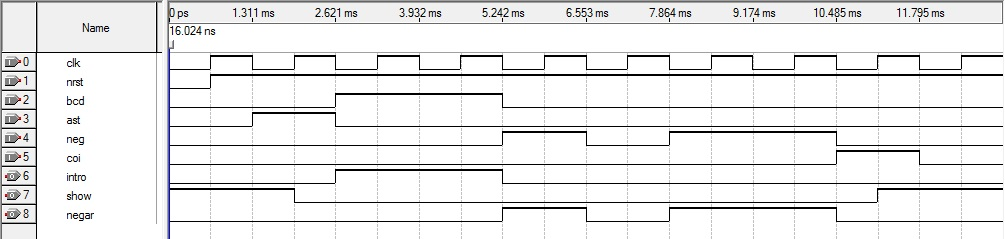
\includegraphics[scale=0.55]{../\projectname/assets/vwf/control.jpg}
  \end{center}
  \caption{\label{fig:sim-\projectname-control} Simulació per al bloc \textsf{control}}
\end{contendfig}

La simulació del bloc es pot veure a la figura~\ref{fig:sim-\projectname-control} (pàgina~\pageref{fig:sim-\projectname-control}).

% FIXME

\vspace{1cm}
